\newlecture
\setcounter{chapter}{10}
\setcounter{section}{0}

%\def\textbookchapter{Chapter 10: Derivatives of Multivariable Functions}
\def\coursetopicnumber{II}
\def\topic{Limits} % this is the printed title
\def\shorttopic{Limits} % short topic
\def\textbookname{Active Calculus} % this is the corresponding textbook
\def\shorttextbookname{AC} % this is the short name for the book
\def\textbooksection{10.1} % corresponding textbook section
\def\textbooksectionurl{https://activecalculus.org/vector/S-10-1-Limits.html} % URL for textbook section
\def\handoutday{} % this is the printed date

%%%%%%%%% DOCUMENT CONTENT STARTS BELOW


\thispagestyle{plain}
\topstuff
\section{\topic{} \booklink{}}
\label{sec:limits}
\subsection{Limits in Calculus I}
Calculus I is all about derivatives of single-variable functions. In order to talk about derivatives, we first need limits!

\begin{defn}[Limit]
    For a function $f(x)$, an $x$ value $a$, and a real number $L$, we say ``the limit of $f(x)$ as $x$ goes to $a$ is $L$,'' written 
    \[
        \phantom{\lim\limits_{x\to a}f(x)=L,}
    \] 
    if the function $f(x)$ gets arbitrarily close to $L$ for all $x$ values sufficiently close to $a$. If no such number $L$ exists, then we say ``the limit of $f(x)$ as $x$ goes to $a$ does not exist (DNE),'' written 
    \[
        \phantom{\lim\limits_{x\to a}f(x) \text{ DNE.}}
    \]
\end{defn}

The key in the definition above is the word ``all.'' The main idea is that $f(x)$ should approach $L$ no matter how one goes to $x=a$. This gives rise to the one-sided limits, $\lim\limits_{x\to a^-}f(x)$ and $\lim\limits_{x\to a^+}f(x)$.

\vspace{.6in}

\begin{ex}
    For $f(x)=\dfrac{|x|}{x}$, compute the following limits:
    %\begin{multicols}{2}
    \begin{enumerate}
        \item $\lim\limits_{x\to 3^-} f(x)$
        \item $\lim\limits_{x\to 3^+} f(x)$
        \item $\lim\limits_{x \to 3}  f(x)$
        \item $\lim\limits_{x\to 0^-} f(x)$
        \item $\lim\limits_{x\to 0^+} f(x)$
        \item $\lim\limits_{x \to 0}  f(x)$
    \end{enumerate}
    %\end{multicols}
\end{ex}

\vfill

\pagebreak 

\begin{defn}[Continuity at a point]
    A function $f(x)$ is \emph{continuous at $x=a$} if
    \begin{multicols}{3}
    \begin{itemize}
        \item \hide{$f(a)$ is defined, }
        \item \hide{$\lim\limits_{x\to a}f(x)$ exists, and}
        \item \hide{$\lim\limits_{x\to a}f(x)=f(a)$.}
    \end{itemize}
    \end{multicols}
\end{defn}

\begin{defn}[Continuity on an interval]
    A function $f(x)$ is \emph{continuous on an interval $I$} if $f(x)$ is continuous at all $x$ values in $I$. (An interval is a subset of $\mathbb{R}$.)
\end{defn}

Basically, this means that the behavior of $f(x)$ near $x=a$ matches with the behavior of $f(x)$ at $x=a$. Graphically, we see this as a connected graph -- one that we can draw without lifting a pen.

\subsection{Limits with multivariable functions}
\begin{defn}[Limit]
    For a function $f(x,y)$, a point $P=(a,b)$, and a real number $L$, we say ``the limit of $f(x,y)$ as $(x,y)$ goes to $(a,b)$ is $L$,'' written 
    \[
        \phantom{\lim\limits_{(x,y)\to(a,b)}f(x,y)=L,}
    \] 
    if the function $f(x,y)$ gets arbitrarily close to $L$ for all points $(x,y)$ sufficiently close to the point $(a,b)$. If no such number $L$ exists, then we say ``the limit of $f(x,y)$ as $(x,y)$ goes to $(a,b)$ does not exist (DNE),'' written
    \[
        \phantom{\lim\limits_{(x,y)\to(a,b)}f(x,y)\text{ DNE}.}
    \]
\end{defn}

As before, the key in the definition above is the word ``all.'' The main idea is that $f(x,y)$ should approach $L$ no matter how one goes to the point $(a,b)$. The difference between now and earlier is that there are so many more ways to approach a point in $\mathbb{R}^2$ than in $\mathbb{R}$!

\vfill

\begin{defn}[Continuity at a point, in a region]
    A function $f(x,y)$ is \emph{continuous at a point $P=(a,b)$} if
    \begin{multicols}{3}
    \begin{itemize}
        \item \hide{$f(a,b)$ is defined,}
        \item \hide{$\lim\limits_{(x,y)\to(a,b)} f(x,y)$ exists, and}
        \item \hide{$\lim\limits_{(x,y)\to(a,b)}f(x,y)=f(a,b)$.}
    \end{itemize}
    \end{multicols}
    A function $f(x,y)$ is \emph{continuous in a region $R$} if $f(x,y)$ is continuous at all points $(x,y)$ in $R$. (A \emph{region} is a subset of $\mathbb{R}^2$.) 
\end{defn}

Basically, this means that the behavior of $f(x,y)$ near $(x,y)=(a,b)$ matches with the behavior of $f(x,y)$ at $(x,y)=(a,b)$. Graphically, we see this as a connected surface, without any jumps or tears.

\pagebreak 

\begin{thm}
    All of our elementary functions (constants, polynomials, rational functions, root functions, trigonometric functions, exponentials, logarithms, inverse trigonometric functions) as well as combinations of them (including addition, subtraction, multiplication, division, exponentiation, and function composition) are continuous wherever they are defined.
\end{thm}

Note: Everything that we're saying here about functions of two variables applies in the same exact way to functions of three variables, of four variables, and so on.
\medskip 

To evaluate $\lim\limits_{(x,y)\to(a,b)}f(x,y)$, if $f(x,y)$ is defined and continuous at the point $(x,y)=(a,b)$, then we can just plug in $x=a$ and $y=b$ and take the result.

\begin{ex}
    Let $f(x,y)=\dfrac{x+y}{x^2+2y^2}$.
    \begin{enumerate}
        \item Evaluate $\lim\limits_{(x,y)\to(3,1)}f(x,y)$. \vfill
        \item Evaluate $\lim\limits_{(x,y)\to(-2,2)}f(x,y)$. \vfill
        \item Are there any points for which we couldn't evaluate the limit here by plugging in?\vfill
    \end{enumerate}
\end{ex}

\subsection{Tricky situations with limits}
There are two situations that make limit evaluation trickier:
\begin{enumerate}
    \item $f(x,y)$ isn't written only in terms of elementary functions. (Often $f(x,y)$ is piecewise-defined, and this includes absolute values.)
    \item $f(x,y)$ isn't defined at $(x,y)=(a,b)$. (This is usually due to division by 0.)
\end{enumerate}
We'll deal mostly with the second case. To handle the limit, we have two techniques.
\begin{itemize}
    \item If we approach the point $(x,y)=(a,b)$ with two different paths in the domain of $f(x,y)$ and get two different results, then the limit does not exist. Note that we can usually evaluate these limits as single-variable limits. We'll see this next, in Section \ref{subsec:different-approaches}.
    \item If we can manipulate $f(x,y)$ algebraically to perform some cancellation, we may be able to directly evaluate the limit. We'll see how to do this in Section \ref{subsec:algebraic-cancellation}.
\end{itemize}

\pagebreak 

\subsection{Different approaches may yield different results}\label{subsec:different-approaches}
If we approach the point $(x,y)=(a,b)$ from two different directions and get two different results, then the limit does not exist.

NOTE: This method will only tell us a limit does not exist. If we get the same result for two different directions, we can't conclude anything. Our primary tool to evaluate a limit is algebraic manipulation. (See the examples that appear after these two examples.)

\begin{ex}
    Let $f(x,y)=\dfrac{x^2+y^2}{x^2+2y^2}$. Compute $\lim\limits_{(x,y)\to(0,0)}f(x,y)$ by computing the limit as $(x,y)$ goes to $(0,0)$ in two different ways: along the $x$-axis; and along the $y$-axis. What can you conclude?
    
    Afterward, compute the limit as $(x,y)$ goes to $(0,0)$ along the line $y=mx$ for constant $m$.
\end{ex}

\vfill

\mbox{} \hfill 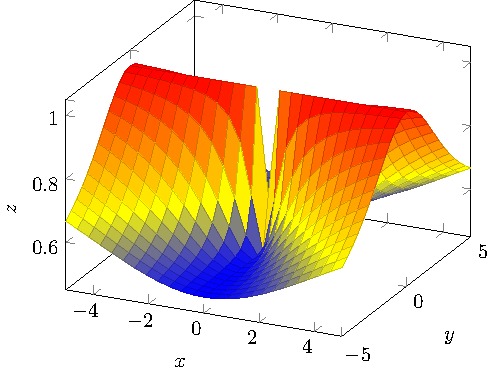
\includegraphics[scale=1]{tikz-pictures/section-10.1-pic1-hole-at-origin.pdf}\label{img:tikz-bad-limit}

\pagebreak 

\begin{ex}
    Let $g(x,y)=\dfrac{x^2y+x^4}{x^4+y^2}$. Compute $\lim\limits_{(x,y)\to(0,0)}g(x,y)$ as $(x,y)$ goes to $(0,0)$ along the line $y=mx$. If that doesn't give a conclusion, try $y=mx^2$.
\end{ex}

\vfill\vfill\vfill

\subsection{Algebra to the rescue}\label{subsec:algebraic-cancellation}
Sometimes, we can use algebraic methods involving factoring and/or conjugates to evaluate limits.
\begin{ex}
    Let $f(x,y)=\dfrac{x^2y-xy}{x-1}$.
    \begin{enumerate}
        \item Evaluate $\lim\limits_{(x,y)\to(0,0)} f(x,y)$.
        \vfill
        \item Evaluate $\lim\limits_{(x,y)\to(1,3)} f(x,y)$.
        \vfill
    \end{enumerate}
\end{ex}

\pagebreak 

\begin{ex}
    Let $g(x,y)=\dfrac{x^2-y^2}{x-y}$. Evaluate $\lim\limits_{(x,y)\to(5,5)}g(x,y)$.
\end{ex}

\vfill

\begin{ex}
    Let $h(x,y)=\dfrac{xy-4y^2}{\sqrt{x}-2\sqrt{y}}$. Evaluate $\lim\limits_{(x,y)\to(4,1)}h(x,y)$.
\end{ex}

\vfill

\pagebreak 
